\documentclass[twoside,12pt]{article}
\usepackage[margin=1in]{geometry}
\usepackage[utf8]{inputenc}
\usepackage{amsmath,amssymb,amsthm}
\usepackage{mathtools}
\usepackage[normalem]{ulem}
\usepackage{enumerate}
\usepackage{graphicx}
\usepackage{hyperref}
\graphicspath{ {images/} }

\DeclareMathOperator{\F}{\mathbb{F}}
\DeclareMathOperator{\Z}{\mathbb{Z}}
\DeclareMathOperator{\N}{\mathbb{N}}
\DeclareMathOperator{\R}{\mathbb{R}}
\DeclareMathOperator{\Q}{\mathbb{Q}}
\DeclareMathOperator{\U}{\mathbb{U}}
\DeclareMathOperator{\id}{\textbf{id}}
\DeclareMathOperator{\inv}{^{-1}}
\DeclareMathOperator{\Po}{\mathcal{P}}
\DeclareMathOperator{\Aut}{\textbf{Aut}}
\DeclareMathOperator{\Hom}{\text{Hom}}
\DeclareMathOperator{\Vect}{\textbf{Vect}}
\DeclareMathOperator{\Gr}{\textbf{Gr}}
\DeclareMathOperator{\im}{\text{im}}
\DeclareMathOperator{\lcm}{\text{lcm}}
\DeclareMathOperator{\varep}{\varepsilon}

\DeclarePairedDelimiter\ceil{\lceil}{\rceil}
\DeclarePairedDelimiter\floor{\lfloor}{\rfloor}
\DeclarePairedDelimiter\abs{\lvert}{\rvert}
\DeclarePairedDelimiter\norm{\lVert}{\rVert}

\makeatletter
\let\oldabs\abs
\def\abs{\@ifstar{\oldabs}{\oldabs*}}
\let\oldnorm\norm
\def\norm{\@ifstar{\oldnorm}{\oldnorm*}}
\let\oldceil\ceil
\def\ceil{\@ifstar{\oldceil}{\oldceil*}}
\let\oldfloor\floor 
\def\floor{\@ifstar{\oldfloor}{\oldfloor*}}
\makeatother

\begin{document}

\noindent \textbf{Sam Goree}

\noindent \textbf{April 2017}

\section*{RTI Exercise 1 Analysis}

\subsection*{Preliminary Analysis}

My first instinct upon examining this dataset was to look at the distributions of all of the attributes independently. Since I'm a visual person, I conducted this analysis by creating bar charts. After that I used association rule mining\footnote{Using the A priori algorithm, implementation at \url{https://github.com/asaini/Apriori}} on a subset of the attributes (age, workclass, education level, married status,occupation, race, sex, hours/week, country and 50k) to identify combinations of attributes that implied other attributes (with confidence over 90\% and support over 20\%). Some observations follow:

\begin{enumerate}
\item This dataset contains considerable skew in a few attributes towards specific values, which may be representative of the US population. For example, 
\begin{itemize}
\item Workclass is skewed towards private (69\%)
\item Race is skewed towards white (86\%)
\item Sex is skewed towards male (67\%)
\item Country is overwhelmingly US (90\%)
\item Most importantly, over 50k is skewed towards under (76\%)
\end{itemize}
These skews are not necessarily an indication that the data gathering metric is faulty, but are definitely something we should watch out for in our analysis, since over-sampling a population could produce false correlations in the data or mislead our classifier, if the test set does not contain similar skews. Especially for the label attribute (over 50k), an unbalanced training set will cause problems for some classifier algorithms.
\item There is a significant amount of missing data for the occupation attribute, but not nearly as much for any other attribute.
\item The relationship attribute puzzles me, it is not described in the readme and has some odd trends, for instance, there are more than 8 times as many husbands as wives. If this is census data, that probably means that wives fill out the form for their household far more often than husbands, or this dataset over-samples gay men in marriages heavily.
\item Notable significant association rules include 
\begin{enumerate}
\item over 50k implies white 90\% of the time
\item private sector and female implies under 50k 91\% of the time
\item never married implies under 50k 95\% of the time
\end{enumerate}
\end{enumerate}

\subsection*{Classifier Results}

I decided to clean some features and remove others to decrease noise before giving it to a classifier. Specifically, I converted the capital gain and capital loss values to a nominal attribute: whether they were zero or not, I converted the country attribute to US or not and removed the education number attribute, since it correlated with the education level attribute. Since the balance of positive to negative examples was so skewed, I elected to experiment with several different ratios of positive to negative examples in the training and test sets to see which resulted in the highest prediction accuracy. I also experimented with three different potential models, random forest, naive bayes and logistic regression classifiers.\footnote{Implementations from scikit-learn \url{http://scikit-learn.org/stable/}}\\

The best model was the logistic regression classifier, which had around 82\% accuracy. In order to handle the unbalanced dataset, I experiment with accuracy values for different fractions of the positive examples in the training set and different ratios between positive and negative examples. Since the other attributes (like sex) indicate that this dataset is not indicative of the US population in general, more research is needed to construct a representative test set. In lieu of one, I balance my test set to have 50\% positive examples and 50\% negative examples. The regression classifier performs best with as much data as possible in the training set, insofar as it maintains balance between positive and negative examples. It is reasonable to assume that given a representative test set, a different ratio of positive to negative examples in the training set would afford higher accuracy.

\begin{table}[ht]

\begin{tabular}{|c|c|c|}
    \hline
    & predicted under 50k & predicted over 50k\\
    \hline
    actual under 50k & 20383 & 2701\\
    \hline
    actual over 50k & 1423 & 3299\\
    \hline
\end{tabular}

\caption{Confusion Matrix for logistic regression classifier}

\end{table}

Rather than include the most informative chart I could find, I decided to include what I found to be the most interesting. Figure 1 shows marital status vs. sex and raises a number of questions. There are over ten times as many husbands as wives, they can't all be married to each other, so where are all of the wives? Why are there four times as many unmarried women as men, despite the dataset being majority male? Are the two people who reported that they are male wives transgender people who are reporting their sex assigned at birth or just errors in the form?

\begin{figure}
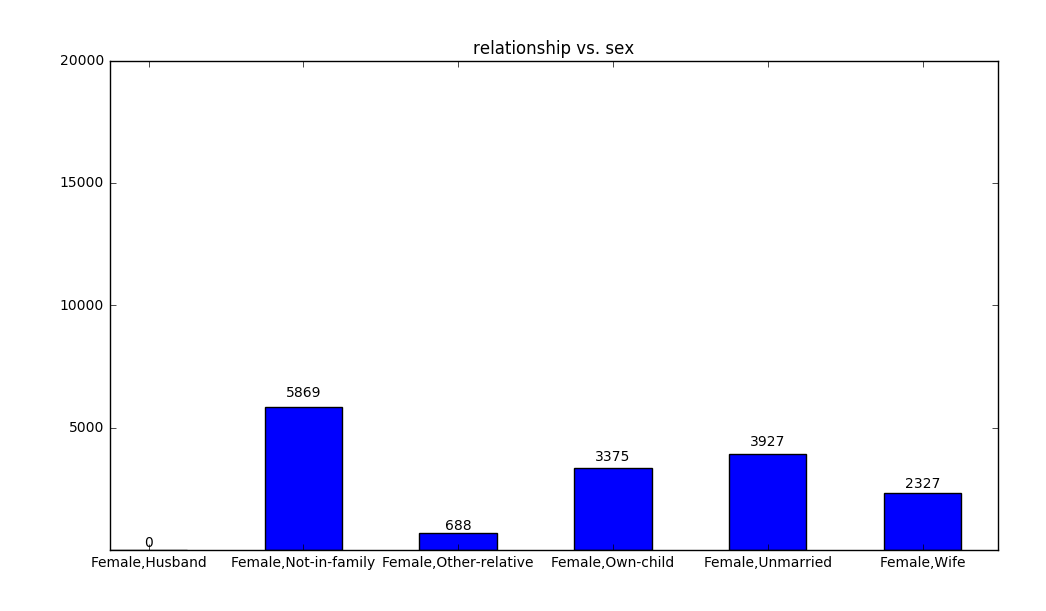
\includegraphics[scale=0.5]{relationship_vs_sex_male.png}
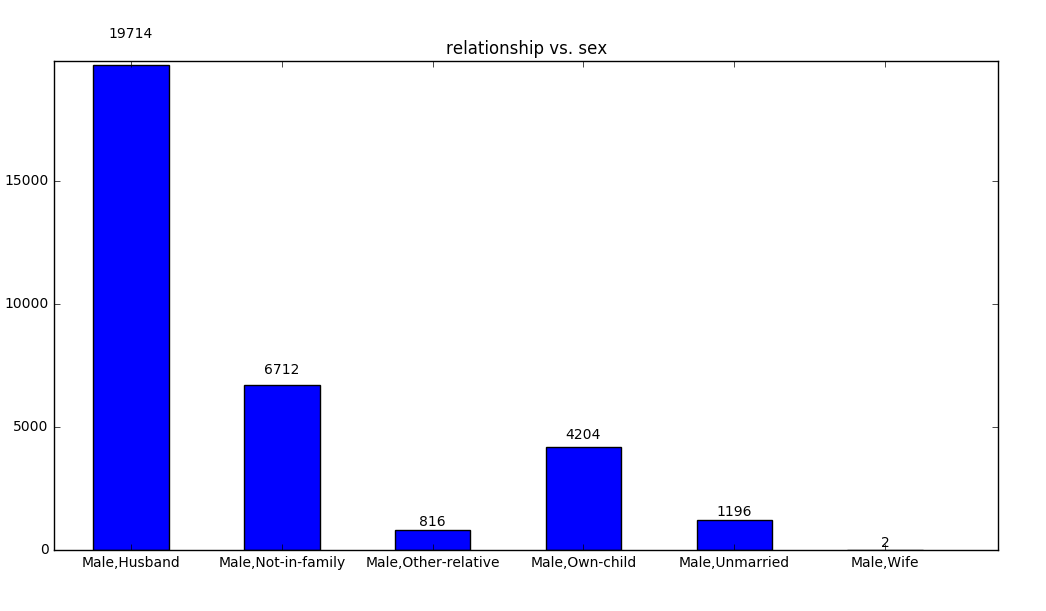
\includegraphics[scale=0.5]{relationship_vs_sex_female.png}
\caption{Intersections of relationship and sex attributes}
\end{figure}

\end{document}